% Template for articles submitted to the International Journal of Forecasting
% Further instructions are available at www.ctan.org/pkg/elsarticle
% You only need to submit the pdf file, not the source files.
% If your article is accepted for publication, you will be asked for the source files.


\documentclass[11pt,3p,review,authoryear]{elsarticle}

\usepackage{listings}
\usepackage{color}
\usepackage{graphicx}
\usepackage{multirow}
\usepackage{array,rotating}

\definecolor{dkgreen}{rgb}{0,0.6,0}
\definecolor{gray}{rgb}{0.5,0.5,0.5}
\definecolor{dkred}{rgb}{0.6,0,0}

\lstset{frame=tb,
  language=R,
  aboveskip=3mm,
  belowskip=3mm,
  showstringspaces=false,
  columns=flexible,
  basicstyle={\small\ttfamily},
  numbers=none,
  numberstyle=\tiny\color{gray},
  keywordstyle=\color{blue},
  commentstyle=\color{dkgreen},
  stringstyle=\color{dkred},
  breaklines=true,
  breakatwhitespace=true,
  tabsize=3
}

\journal{International Journal of Forecasting}
\bibliographystyle{model5-names}
\biboptions{longnamesfirst}
% Please use \citet and \citep for citations.


\begin{document}

\begin{frontmatter}

\title{Fast and Accurate Forecasting on Yearly Time Series with Forecast Combinations}

%% AUTHORS %%%%%%%%%%%%%%%%%%%%%%%%%%%%%%%%%%%%%%%%%%%%%%%%%%%%%%%%%%%%%%%%%%%%
%% Leave this section commented out so that the paper is blinded for review.
%% Group authors per affiliation:
% \author[ss]{David Shaub\corref{cor}}
% \address[ss]{Harvard University Extension School}


%% Only give the email address of the corresponding author
% \cortext[cor]{Corresponding author}
% \ead{davidshaub@g.harvard.edu}
%%%%%%%%%%%%%%%%%%%%%%%%%%%%%%%%%%%%%%%%%%%%%%%%%%%%%%%%%%%%%%%%%%%%%%%%%%%%%%%%


\begin{abstract}
Combination forecasting strategies have long been known to produce superior out-of-sample forecasting performance relative to even its best single component models. In the M4 forecasting competition, this approach was harnessed to produce a very simple forecast combination strategy that achieved competitive performance on yearly time series. An analysis of the ensemble model versus the component models suggests the competitive accuracy comes from avoiding poor forecasts instead of beating the best individual models. Moreover, the model fits very quickly, can easily scale horizontally with additional CPU cores or machines, and can very quickly and easily be implemented by users. This approach might be of particular interest to users who need accurate yearly forecasts without significant time, resources, or expertise to tune models. Users of the R statistical programming language can access this model in the "forecastHybrid" package.
\end{abstract}

\begin{keyword}
Automatic forecasting\sep Combining forecasts\sep Evaluating forecasts\sep Forecasting competitions\sep Software
% Suggested keywords are listed at https://ijf.forecasters.org/keywords/
\end{keyword}

\end{frontmatter}


\section{Introduction}
Model selection presents a challenge for forecasters since selecting the incorrect model leads to additional forecasting error. One hedge against incorrect model specification is the combination of forecasts from several candidate models. Granger \& Bates \cite{BatesGranger1969} first suggested such an approach and observed that somewhat surprisingly the combined forecast can even outperform that single best performing component forecast. While combination weights selected equally or proportionally to past model error are possible approaches, no shortage of combination schemes have been suggested. For example, instead of normalizing weights to sum to unity, unconstrained--and even negative--weights could be possible \citep{GrangerRamanathan1984}.

It would appear that the simplest approach of assigning equal weights to all component models is woefully obsolete and likely noncompetitive compared to the multitude of sophisticated combination approaches. However, results from the 2018 M4 competition show that such a simple approach can still be competitive, particularly for yearly time series where the method achieved 3rd place.

This article is organized as follows: section 2 describes the combination methodology, section 3 contains analysis of the performance characteristics of this model in the M4 competition versus individual models, and section 4 concludes.

\section{Methodology}
The combination strategy employed in the M4 competition submission utilized the statistical programming language R \citep{Rlang} and leveraged the "forecastHybrid" \citep{forecastHybrid} package. The component models allowed in the "forecastHybrid" package are the  \lstinline{auto.arima()}, \lstinline{ets()}, \lstinline{thetaf()}, \lstinline{nnetar()}, \lstinline{stlm()}, \lstinline{tbats()}, and \lstinline{snaive()} models provided in "forecast" package \citep{Forecast}.


The following R code produces this forecast combination for a single yearly time series \lstinline{x} and a forecasting horizon \lstinline{h = 6} along with 95\% prediction intervals.
\begin{lstlisting}[language=R]
forecastM4 <- function(x, h = 6){
    return(forecast(hybridModel(x, models = "aft", verbose = FALSE),
                      h = h, level = 95, PI.combination = "mean"))
}
\end{lstlisting}

\section{Analysis}
We might reasonably question why such a simple and well-known technique of averaging forecasts proved competitive in the M4 yearly series. One hypothesis is that model selection is a difficult problem and more complex forecasting methodologies struggle to select a model that will perform well in the forecasting horizon. The model selection problem for complex models could manifest itself as either the explicit selection between a candidate pool of models (or the weights assigned to these models if using more than one) or the implicit problem of selecting the optimal hyperparameters if a single model is used that has many possible tuning parameters such as neural networks. The examination that follows supports this hypothesis and shows that the mean ensemble approach achieves competitive performance not by producing forecasts that barely miss the actual values but rather by producing fewer forecasts that very badly miss the actual values.

The MASE produced by the simple ensembling procedure on yearly M4 data will be compared against two other forecasting methods for each time series in the M4 yearly data. In the first method, a model selection procedure chooses from the individual component \texttt{auto.arima())}, \texttt{thetam())}, and \texttt{tbats())} models by forming a holdout set on the M4 training data of size equal to the forecasting horizon 6 and selecting the model that minimizes MASE on this holdout set. That model is then retrained on the whole train set before producing forecasts on the M4 holdout set. This method will be called the best component model approach. In the second method, we will instead assume an oracle has selected the individual component model that performs best on the M4 test set. Outperforming such an oracle model selection procedure is a very difficult task, but this will serve as a benchmark to evaluate the model selection procedure and to determine if the ensemble achieves its forecasting strength through beating this standard or through avoiding selecting poor component models.

% table with results will go here
% histogram showing distribution of best, average, and oracle models MASE will go here

\begin{figure}[h]
\centering
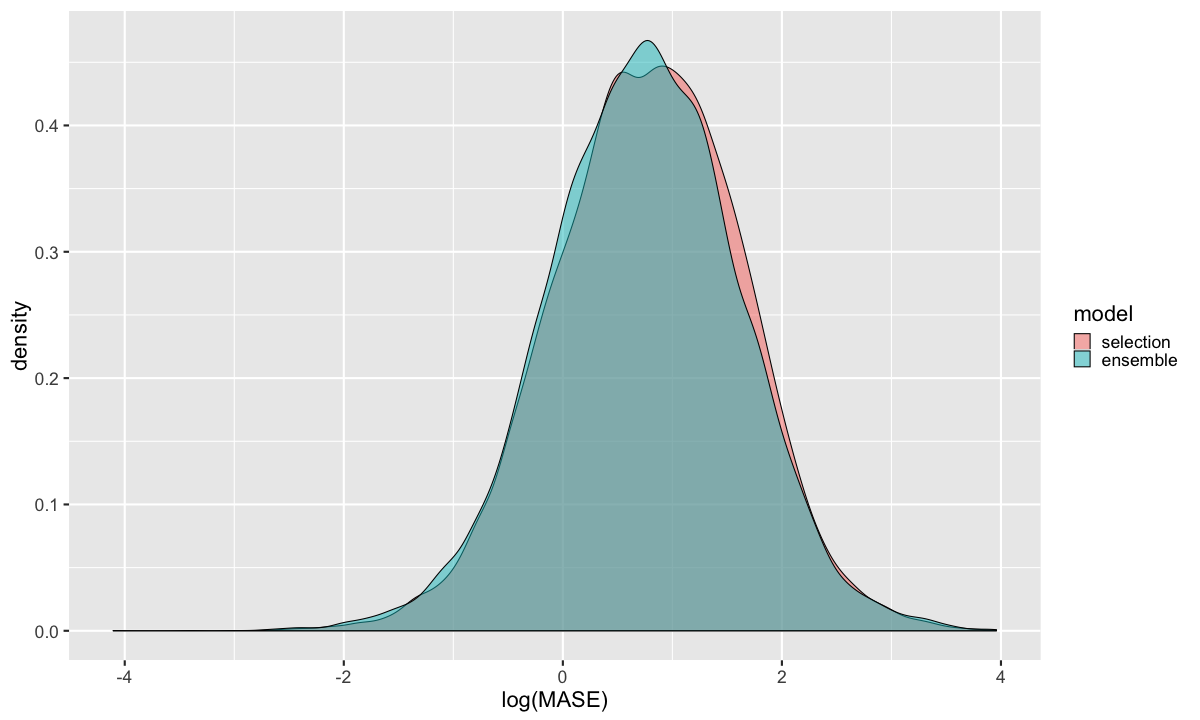
\includegraphics[width=1.0\textwidth]{distribution}
\caption{Distribution of MASE for the ensemble and model selection forecasting procedures}
\end{figure}

% Table of Oracle model selection and best individual model
% latex table generated in R 3.5.1 by xtable 1.8-3 package
% Sat Oct  6 19:24:20 2018
\begin{table}[ht]
\centering
\begin{tabular}{rrrr}
  \hline
  & \multicolumn{3}{c}{\textbf{Reference}} \\
 \textbf{Selected} & Arima & BATS & Theta  \\
 \hline
 Arima & 1397 & 1486 & 1935 \\ 
   BATS & 1213 & 1197 & 1450 \\ 
  Theta & 4491 & 4613 & 5218 \\ 
   \hline
\end{tabular}
\caption{Reference best individual model on test set versus model from selection procedure}
\end{table}

\section{Conclusion}
It might sound trivial to state that the way to produce good forecasts is to avoid making bad forecasts, but sophisticated models have great difficulty avoiding making bad forecasts. An examination of a simple ensemble forecasting method shows that equal arithmetic averaging of base models can serve of a hedge of risk.

\section*{Acknowledgments}

This research did not receive any specific grant from funding agencies in the public, commercial, or not-for-profit sectors.


% Bibliography.
\section{References}
\bibliography{forecastHybrid}
\end{document}
